\chapter{Data Management \hideme{Steve Timm and Robert Illingworth} }
\label{ch:datamgmt}

%%%%%%%%%%%%%%%%%%%%%%%%%%%%%%%%
\section{Introduction}
\label{sec:datamgmt:xyz}  %% fix label according to section

The Data Management subsystem serves the function of bringing data from the detectors to the archival storage facility 
and then distributing it to storage elements around the world.  The components include a data ingest manager, a
replica manager that knows the location of files and manages the transfers between storage element, a metadata 
catalog that keeps track of the types and provenance of data, and an interface to deliver the appropriate files 
to the workflow management system and interactive users.

DUNE Data Management is currently in the process of deploying several new components in the Data Management
system, to replace the legacy SAM system which currently does the function of replica manager, metadata server, 
and file delivery.  The goal is to have the new system in place before beam running begins on ProtoDUNE-II
(single-phase horizontal drift).  

\todo{Need to insert basic data management architecture here}

\begin{figure}[ht]
    \centering
%\includegraphics[height=6cm]{graphics/DataManagement/Figures/data_management_diagram.pdf}
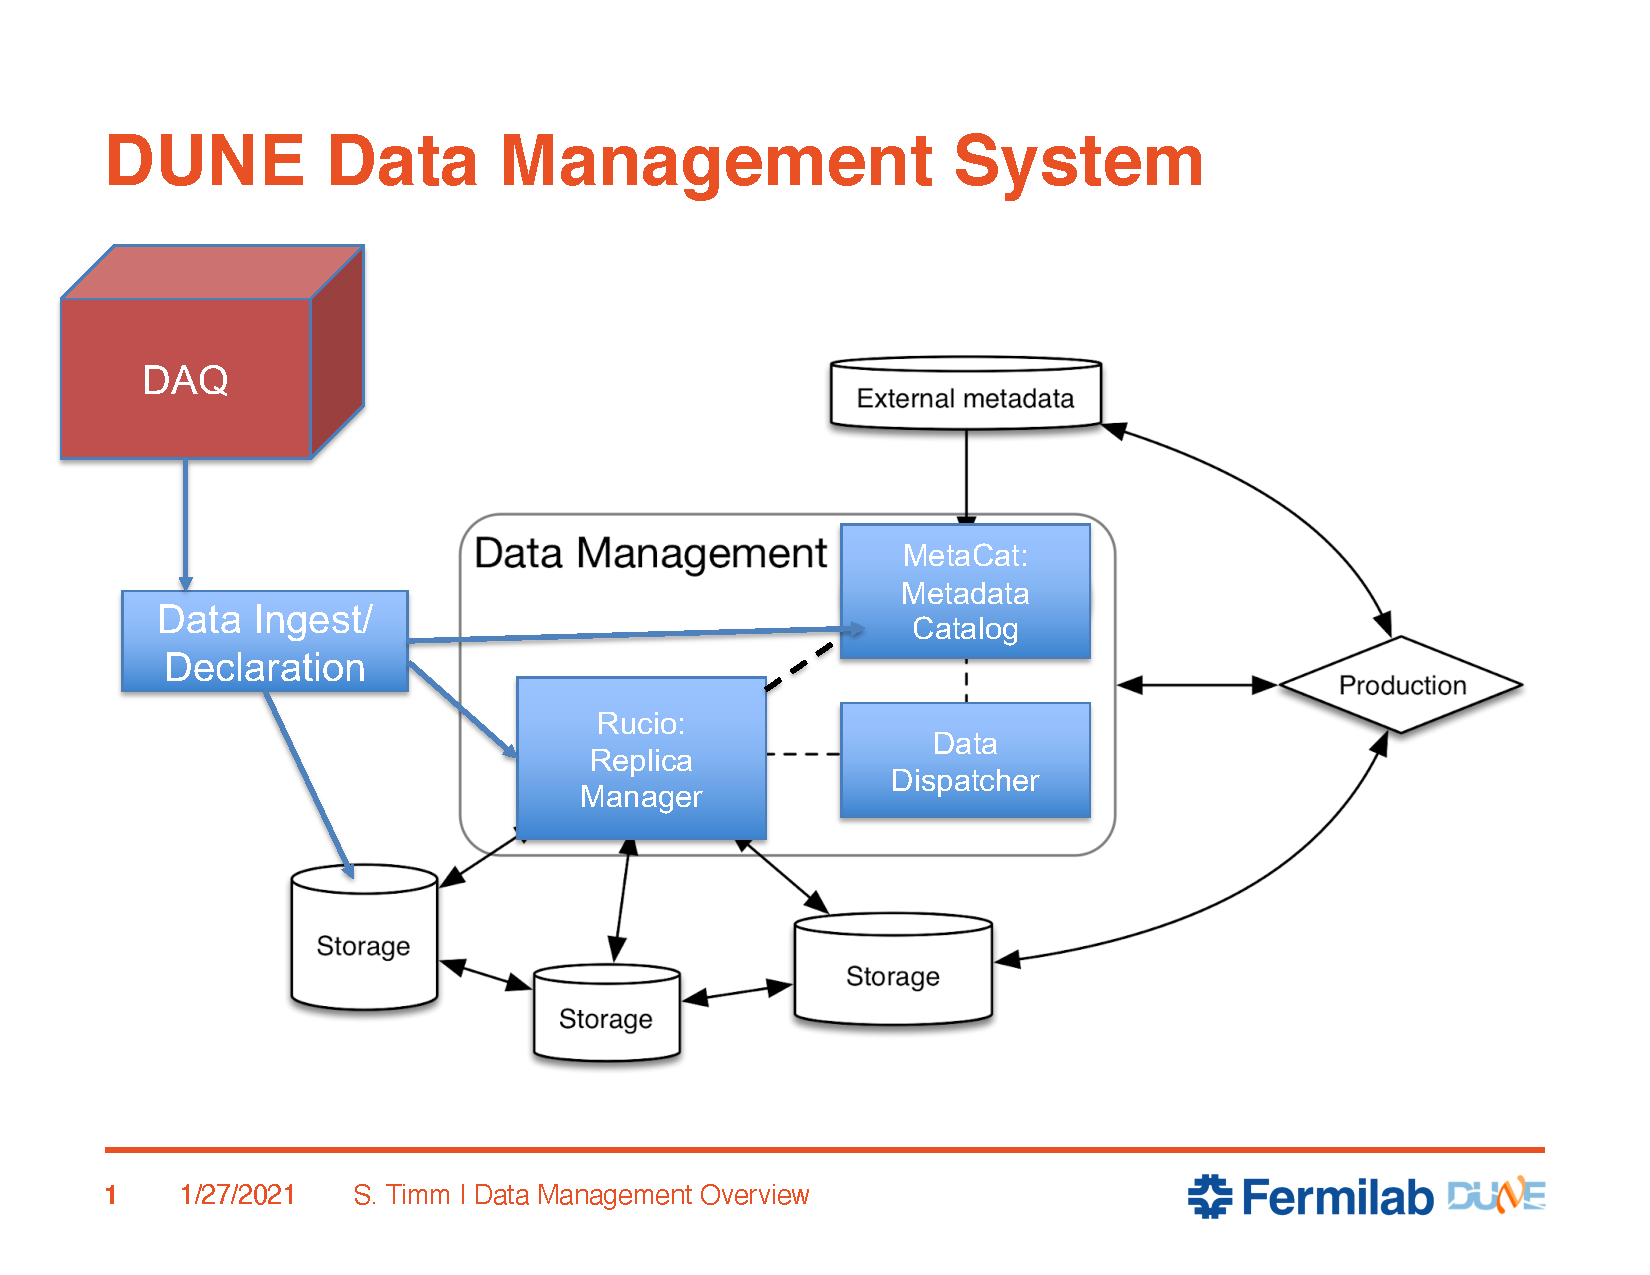
\includegraphics[height=8cm]{graphics/DataManagement/data_mgmt_diagram.pdf}
    \caption{Data Management Architecture Diagram}
    \label{fig:datamanagement}
\end{figure}


\section{Data Ingest Manager}

The Data Ingest Manager will run at detector sites.  It consists of two components:  the Ingest Daemon and the Declaration Daemon.  The Ingest Daemon will 
run within the detector hall, detect new files in the data store, extract the metadata and add new metadata fields
if necessary, calculate the checksum of the files, initiate and monitor the transfers to the first managed 
storage element, and send a signal back to the DAQ when the file has been transferred and can be deleted from the data store.
Files will be transferred to a dropbox on the nearest managed storage element, using FTS3 as the transport mechanism.  
The Declaration Daemon will run on or near a storage element that is managed by the replica manager. 
It will detect new files that have been added to the dropbox, and declare them to the metadata catalog and the replica manager.  It will then instruct the replica manager to send these files to permanent tape-backed storage and monitor the transfer to be sure that this has been done, and then send a signal to remove them from the temporary dropbox.

These daemons will be performing most of the functions that the current data transport system does, they only 
require modification to contact the new replica manager and metadata catalog rather than the current ones.  The 
requirements for these daemons have been defined and we expect coding work to start in mid to late summer 2021.

\section{Replica Manager}

The replica manager has the functionality of tracking where all data files are located and ensuring that they 
are moved from point to point as needed.  The choice that we have made for this functionality is the Rucio data
management system.  This system was originally developed by the ATLAS experiment and has now been deployed to 
a number of other HEP and astronomy experiments.  DUNE has had a Rucio server since 2019.  All raw data that was
taken in the fall 2018 ProtoDUNE-SP (NP04) run and since that time, as well as all raw data taken by the ProtoDUNE-DP (NP02) run, is tracked by Rucio.

Rucio is a rule-based system.  Files are sent to remote servers and kept there based on a system of rules
that are created by the experiment data managers.  Data can be accessed interactively or in batch jobs and
Rucio has a built-in system of delivering the URI of the closest replica to the running job for access via streaming.

The main work that remains to be done in implementing the Rucio server is the process of back-loading all relevant 
data in the legacy SAM system into Rucio as well.  Currently about 50\% of the data by volume is known by Rucio but only about 25\% of the files by file count are declared to Rucio at the moment.  This is the largest current 
operational issue under way.

There are also some key features that we need from the Rucio developers.  One of them is the capacity to 
do the logical to physical file name mapping on our tape sites, based on the metadata of the file.  Another
is the hook that requires that any file that is declared to Rucio is also declared to the metadata catalog.

Rucio has a rudimentary internal metadata functionality but it is not used by any of the main 
experiments that use it.  We thought it wise for DUNE to also have a 
\section{Metadata Catalog}



\section{Data Dispatcher}

\section{Tools}


